\subsection{CONFIGURACIÓN ARCHIVO INICIAL}
El proyecto contendrá un nodo raíz el cual será el que tendrá los llamados al conjunto de elementos que tendrá nuestra librería. Anteriormente se creó un directorio llamado “src” en la raíz de “crown”, dentro de “src” debemos crear un archivo llamado “index.js” este es un archivo de JAVASCRPT el cual definiremos como punto de inicio de webpack  y a partir de este buscará todas las importaciones de otros submódulos. Con el siguiente comando creamos el archivo requerido.
\newline
\newline
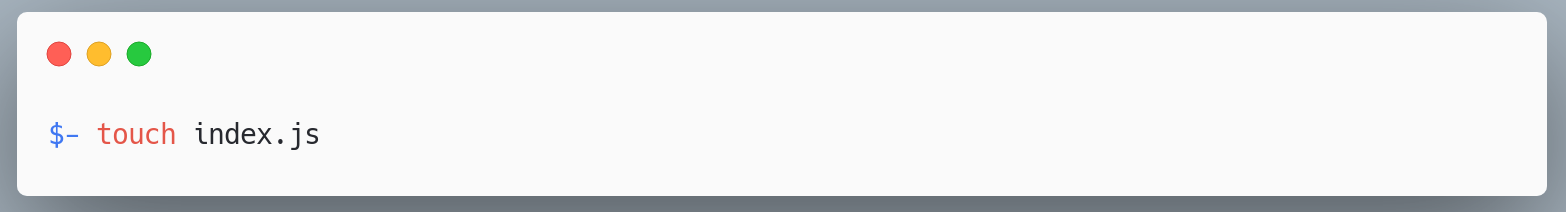
\includegraphics[width=1\textwidth]{./Imagenes/carbon.png}
\newline
Dentro de este archivo debemos poner el llamado a cada elemento que se vaya agregando a nuestra librería ( Botones, Campos de texto, Tablas etc.), en la siguiente ilustración se muestra la manera en que se deben agregar los elementos.
\newline
\newline
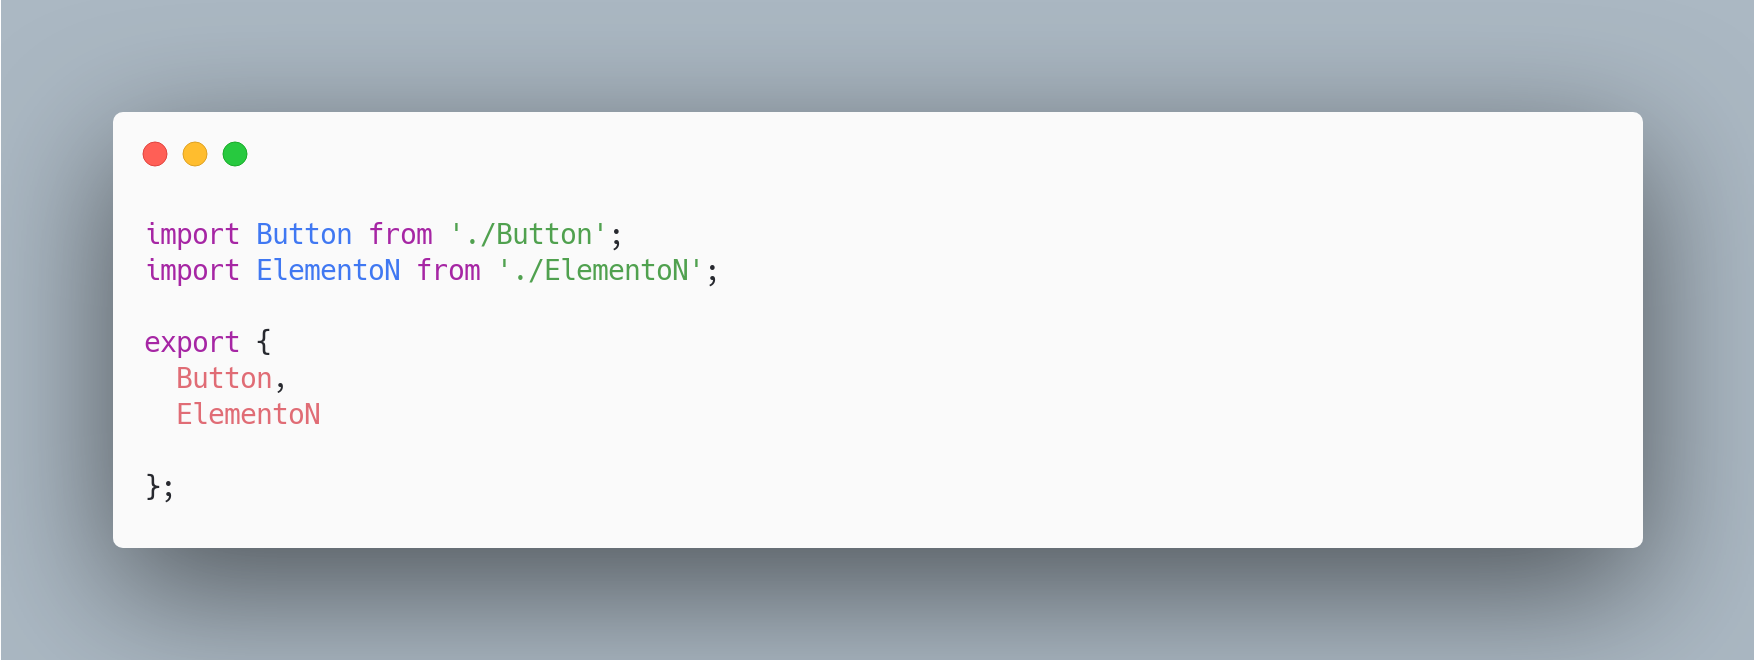
\includegraphics[width=1\textwidth]{./Imagenes/carbon-2.png}
\newline
El primer bloque de código muestra la importación de cada uno de los elementos a nuestro archivo index, y la segunda parte exportamos un objeto de JAVASCRIPT con cada uno de los elementos.
WEBPACK analiza cada elemento que se incluye en el objeto y busca el contenido existente dentro de cada uno.
Cada uno de los elementos que se necesita agregar deben estar situados a la misma altura del archivo “index.js” esto dentro del directorio “src” para que puedan ser procesados.

\subsection{ELEMENTO BOTÓN}
El primer elemento que vamos a agregar es el botón, para esto creamos un directorio llamado “Botton” de la siguiente manera.
\newline
\newline
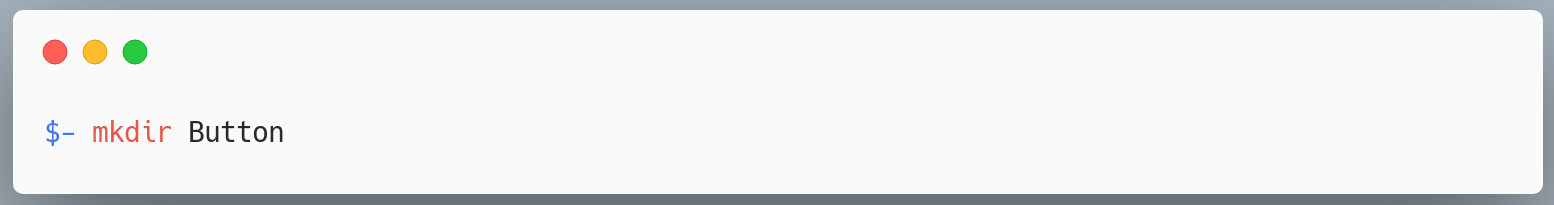
\includegraphics[width=1\textwidth]{./Imagenes/carbon-3.png}
\newline
Y dentro de este directorio crearemos dos archivo que son los que incluirán el núcleo de nuestro botón, el primer archivo se llamará “index.js ” esto es así ya que por defecto, cuando importas un archivo que está dentro de un directorio, JAVASCRIPT toma el que es llamado “index.js” y no es necesario especificar este dato, esto lo podemos ver de manera clara en el archivo inicial “index.js” que está al mismo nivel que el directorio “Botton”, el cual importa el elemento Botton pero no especifica el archivo. Este archivo solamente hace el llamado al segundo archivo “Botton.js” que es el que tiene el código fuente del botón. 
\newline
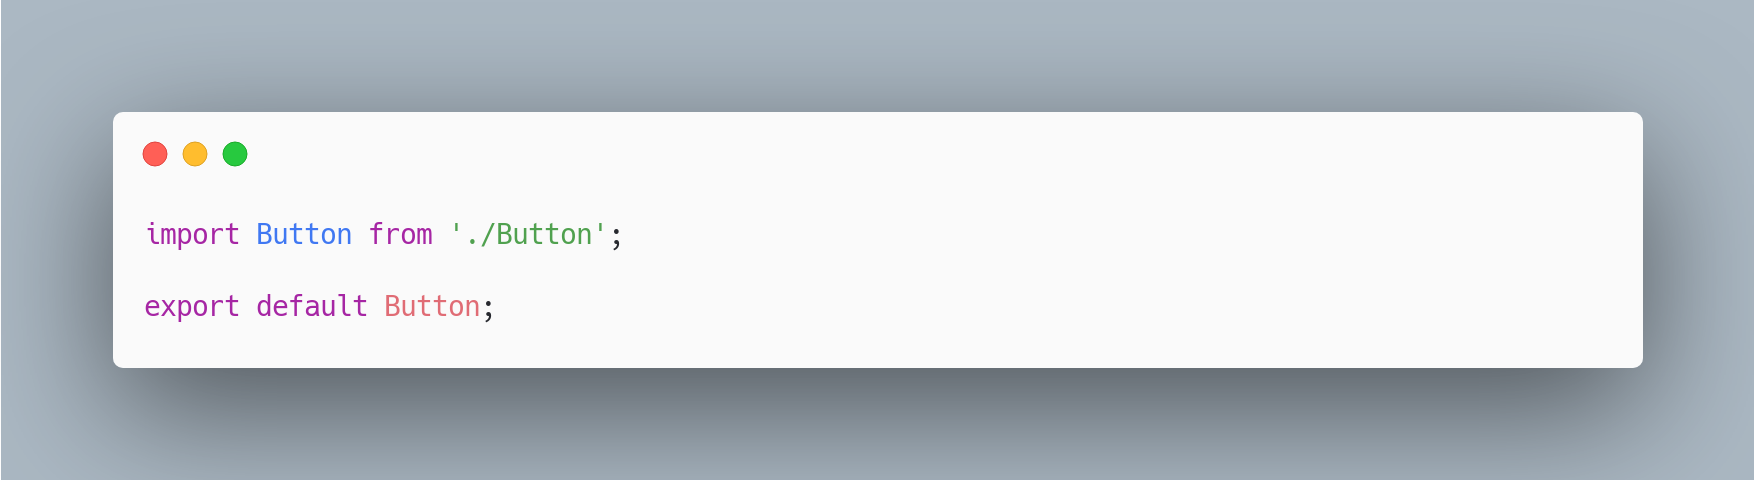
\includegraphics[width=1\textwidth]{./Imagenes/carbon-5.png}
\newline
El segundo archivo ya mencionado “Botton.js”  hace el render de nuestro botón, y gestiona la configuración que el usuario final quiera asignarle.
En la siguiente tabla se muestran los props ( configuración inicial  ) del botón.
\begin{center}
 \begin{tabular}{|c|c|c|c|} 
 \hline
Nombre & Uso &  Tipo de dato & Valor por defecto\\ [0.5ex] 
 \hline\hline
text & Texto que mostrará el botón.  &  Cadena de texto. & Click me! \\  [2.5ex] 
 \hline
onClick & Es la función que ejecutará cuando se hace click. & Funcion. & Función vacía. \\[2.5ex] 
 \hline
color &  Es el color del botón. & Cadena de texto. & --blue-4 \\[3.5ex] 
 \hline
 textColor & Es el color del texto en el botón. &  Cadena de texto. & --white \\[2.5ex] 
 \hline
borderColor & Es el color del borde del botón. & Cadena de texto. & --blue-4 \\ [2.5ex] 
 \hline
\end{tabular}
\end{center}
Los colores que se usan son una constante definida por la librería ya que se considera que son cromáticamente compatibles entre ellos, este tema se abordará más adelante.
A continuación se muestra un fragmento del código que permite agregar la configuración requerida.
\newline
\newline
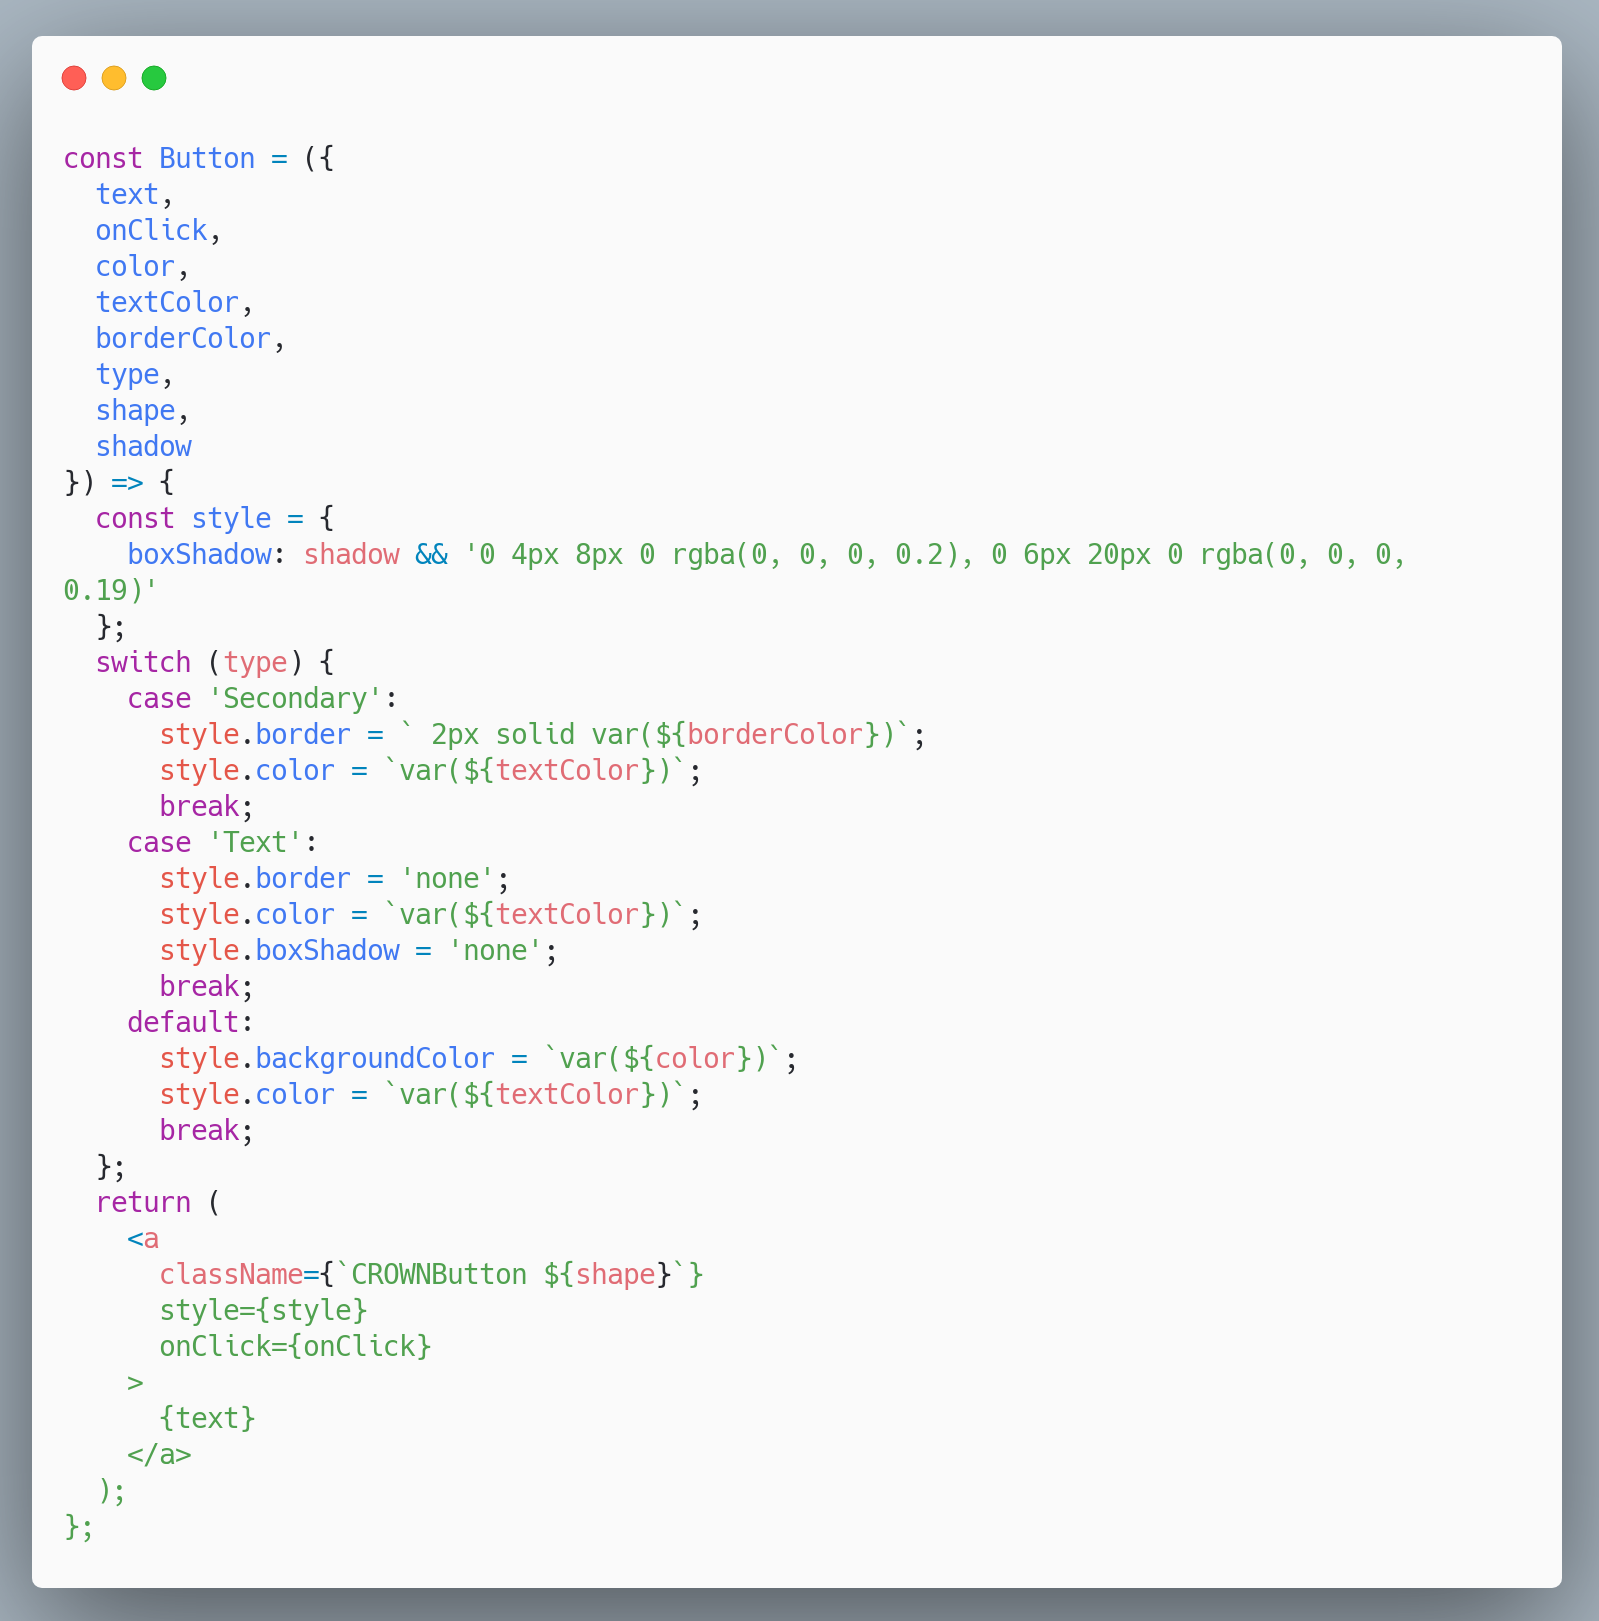
\includegraphics[width=1\textwidth]{./Imagenes/carbon-9.png}
\newline
En la primera parte podemos ver una lista de la configuración dada,  después definimos un objeto llamado styles el cual agrega dentro de un switch el CSS para que sea mostrado de acuerdo al tipo ( type ) de botón que se quiere. Finalmente regresa HTML el cual es nuestro botón configurado.
Se puede observar que dentro de la etiqueta <a> tenemos “className” esto agrega la clase en la cual definiremos el CSS.
Dentro del archivo CSS agregamos el diseño base de nuestro botón, aquí tenemos el  tamaño de la letra, tamaño del botón, grosor de letra y otras cosas más.
\newline
\newline
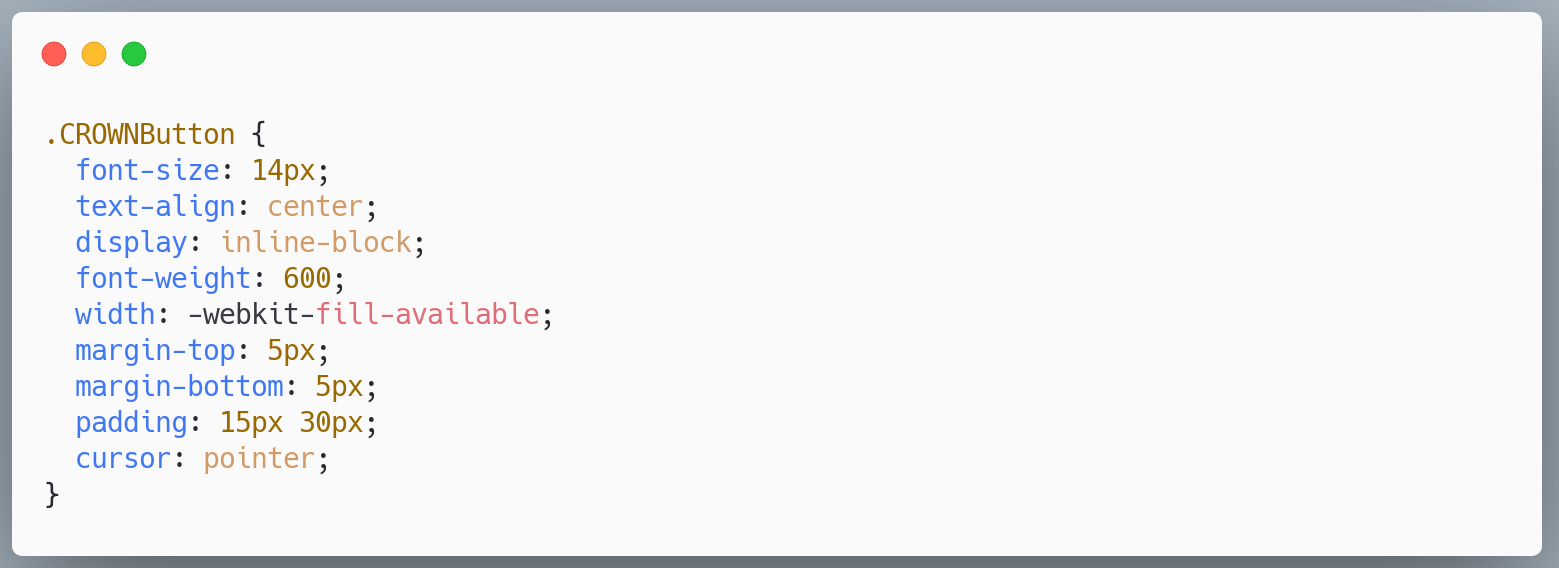
\includegraphics[width=1\textwidth]{./Imagenes/image26.png}
\newline



